\begin{figure}[tb]
  \centering
  \begin{subfigure}{0.31\linewidth}
 %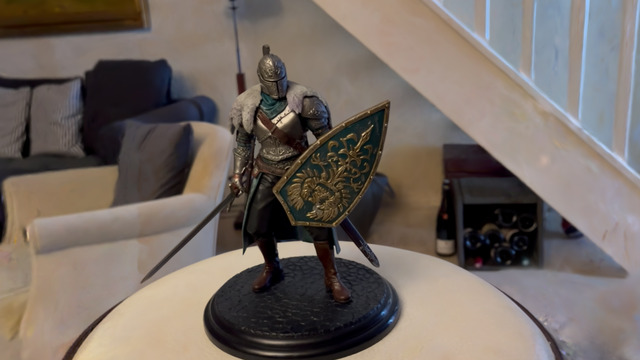
\includegraphics[trim={12cm 0 15cm 0},clip,width=\linewidth]{images/edition/faraam0_rgb_166.png}
 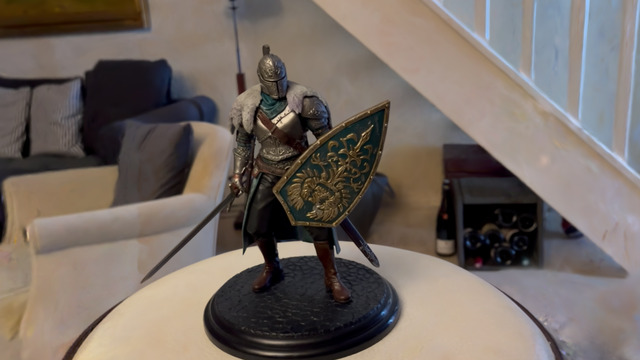
\includegraphics[trim={4cm 0 5cm 0},clip,width=\linewidth]{images/edition/faraam0_rgb_166.jpg}
 \caption{Original pose}
  \end{subfigure}
  %
  \hfill
  %
  \begin{subfigure}{0.31\linewidth}
  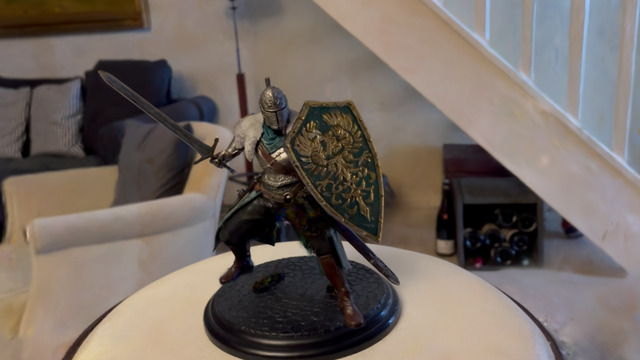
\includegraphics[trim={4cm 0 5cm 0},clip,width=\linewidth]{images/edition/faraam0_rgb_64.jpg}
  \caption{Edited pose}
  \end{subfigure}
  %
  \hfill
  \begin{subfigure}{0.31\linewidth}
  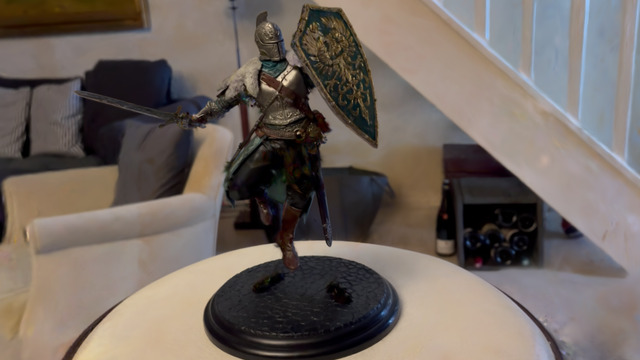
\includegraphics[trim={4cm 0 5cm 0},clip,width=\linewidth]{images/edition/faraam0_rgb_64_1.jpg}
  \caption{Edited pose}
  \end{subfigure}
  %
  \caption{
  \textbf{Examples of animation with Frosting.} We were able to animate the sculpture in the left image using the rigging tool in Blender.
  }
  \label{fig:edition-examples}
\end{figure}